\documentclass[12pt]{article}
\usepackage{graphicx} % Required for inserting images
\usepackage[spanish]{babel}
\usepackage{lmodern}
\renewcommand{\familydefault}{\sfdefault}
\usepackage{geometry}
\usepackage{setspace}
\usepackage{float}
\usepackage{xcolor}
\usepackage{amsmath}
\usepackage{tikz}
\usepackage[colorlinks=true, urlcolor=blue]{hyperref}
\usepackage{hyperref}
\title{Practica 2 - WEB}
\author{Cerón Samperio Lizeth Montserrat}
\date{September 2025}

\begin{document}
\definecolor{azul}{RGB}{0, 168, 255}
\definecolor{azul2}{RGB}{7, 74, 163}

\begin{titlepage}
    \thispagestyle{empty}
    \newgeometry{left=2cm, right=1cm, top=2cm, bottom=2cm}
    
    % Gráfico de fondo corregido para ser fiable
    \begin{tikzpicture}[overlay, remember picture, fill opacity=0.7]
        \begin{scope}[shift={(current page.center)}]
            \rotatebox{-45}{\fill[azul2] (5, -15) rectangle (12, 15);}
            \rotatebox{-45}{\fill[azul] (3, -15) rectangle (5, 15);}
        \end{scope}
    \end{tikzpicture}
    
    \begin{spacing}{1.5}
        {\Huge \bfseries \noindent PRÁCTICA 2}
        \vspace{10pt}

        {\LARGE MÉTODOS HTTP: PUT, PATCH, DELETE, GET}
        
        \vspace{1cm}
        
        {\Large Equipo:} \\
        {\Large Beltrán Saucedo Axel Alejandro} \\
        {\Large Cerón Samperio Lizeth Montserrat} \\
        {\Large Higuera Pineda Angel Abraham} \\
        {\Large Lorenzo Silva Abad Rey} \\
        {\Large 4BV1}
    \end{spacing}
    
    \vspace{1.5cm}

    \begin{minipage}{7.5cm} % Ancho ajustado
        {\Large ESCUELA SUPERIOR DE CÓMPUTO}
    \end{minipage}

    \vfill % Empuja el contenido hacia el final de la página

    \begin{flushleft}
        {\Large \color{black}
        % Comando \textbf corregido con llaves
        \textbf{TECNOLOGÍAS PARA EL DESARROLLO DE APLICACIONES WEB}}
        
        \vspace{0.5cm}
        
        25/09/2025
    \end{flushleft}
    \vspace{1cm}
\end{titlepage}


\section{Introducción}
\subsection*{Objetivo de la práctica:}
El objetivo de la práctica es implementar los métodos HTTP: PUT, PATCH, GET, DELETE en Python con FastAPI, también realizar pruebas de cada uno de los métodos, poniendo a prueba las respuestas que brindará. La aplicación simulará la gestión de paquetes, es decir, que se puede crear un item nuevo con peso y valor, también se le puede poner un ID para ejecutar las funciones de borrar y actualizar parcialmente por el ID. \\


\subsection*{Métodos HTTP:}
\begin{itemize}
    \item \textbf{GET:} Este método se utiliza para solicitar datos de un recurso específico. En la práctica, se implementa para obtener la lista completa de paquetes o un paquete específico por su ID.
    \item \textbf{POST:} Este método se utiliza para enviar datos a un servidor para crear un nuevo recurso. En la práctica, se implementa para crear un nuevo paquete con atributos como peso y valor.
    \item \textbf{PUT:} Este método se utiliza para actualizar completamente un recurso existente. En la práctica, se implementa para actualizar todos los atributos de un paquete específico identificado por su ID.
    \item \textbf{PATCH:} Este método se utiliza para actualizar parcialmente un recurso existente. En la práctica, se implementa para modificar solo algunos atributos de un paquete específico identificado por su ID.
    \item \textbf{DELETE:} Este método se utiliza para eliminar un recurso específico. En la práctica, se implementa para eliminar un paquete identificado por su ID. \cite{ref1}
\end{itemize}

\section{Fundamentos teoricos}
\subsection*{FastAPI:}
FastAPI es un framework web para construir APIs en Python, lanzado en diciembre de 2018 por Sebastián Ramírez, un desarrollador colombiano. Está diseñado para ser:
\begin{itemize}
    \item \textbf{Rápido:} comparable en rendimiento a Node.js y Go gracias a su base en ASGI (Asynchronous Server Gateway Interface).
    \item \textbf{Moderno:} aprovecha las anotaciones de tipo de Python 3.6  
    \item \textbf{Automático:} genera documentación interactiva con Swagger UI y ReDoc.
    \item \textbf{Seguro y robusto:} ideal para APIs que requieren validación estricta y autentic
\end{itemize}
Pero,  ¿qué hace realmente FastAPI?

Nos permite crear endpoints o rutas para nuestra API, que pueden ser accedidas mediante los diferentes metodos HTTP, como GET, POST, PUT, DELETE, entre otros.\\
Además nos permite:
\begin{itemize}
    \item Validar automaticamente los datos de entrada y salida utilizando Pydantic.
    \item Servir modelos de machine learning en producción. 
    \item Integrarse facilmente con base de datos, etc.
    \item Generar documentación interactiva sin esfuerzo.
\end{itemize}

Pero, ¿para qué lo usamos realmente?\\
Usamos FastAPI para crear aplicaciones que se comunican por internet, como por ejemplo:
\begin{itemize}
    \item Aplicaciones web que mandan y reciben datos (como una app de clima o una tienda en línea).
    \item Sistemas que conectan con modelos de inteligencia artificial (como chatbots o análisis de imágenes).
    \item Servicios que otras apps usan para pedir información (como “dame los datos del usuario” o “guárdame esta foto”).
\end{itemize}

\subsection*{HTTP:}
FastAPI utiliza HTTP para comunicarase entre la aplicación web y el cliente. Cada vez que alguien hace una petición (Por ejemplo: GET, POST, etc) a nuestra API, FastAPI recibe esa petición, la procesa y responde con los datos solicitados.\\

¿Qué es HTTP?\\
HTTP (Hypertext Transfer Protocol). Es un lenaguaje utilziado para realizar una comunicación entre un cliente (como un navegador web o una app móvil) y un servidor (donde vive la aplicación web).\\
Funciona con peticiones y respuestas, aglunas de ellas son:
\begin{itemize}
    \item \textbf{GET:} Solicita datos de un recurso específico.
    \item \textbf{POST:} Envía datos para crear un nuevo recurso.
    \item \textbf{PUT:} Actualiza completamente un recurso existente.
    \item \textbf{PATCH:} Actualiza parcialmente un recurso existente.
    \item \textbf{DELETE:} Elimina un recurso específico.
\end{itemize}

Tambien se cuentan con las HTTP Exceptions, que son respuestas a errores que ocurren cuando algo sale mal en la comunicación entre el cliente y el servidor.\\
Algunos ejemplos son:
\begin{itemize}
    \item \textbf{404:} No encontrado
    \item \textbf{403:} Prhohibido
    \item \textbf{500:} Error interno del servidor
    \item \textbf{400:} Solicitud incorrecta  
\end{itemize}

\section{Diagrama UML}
\begin{figure}[H]
    \centering
    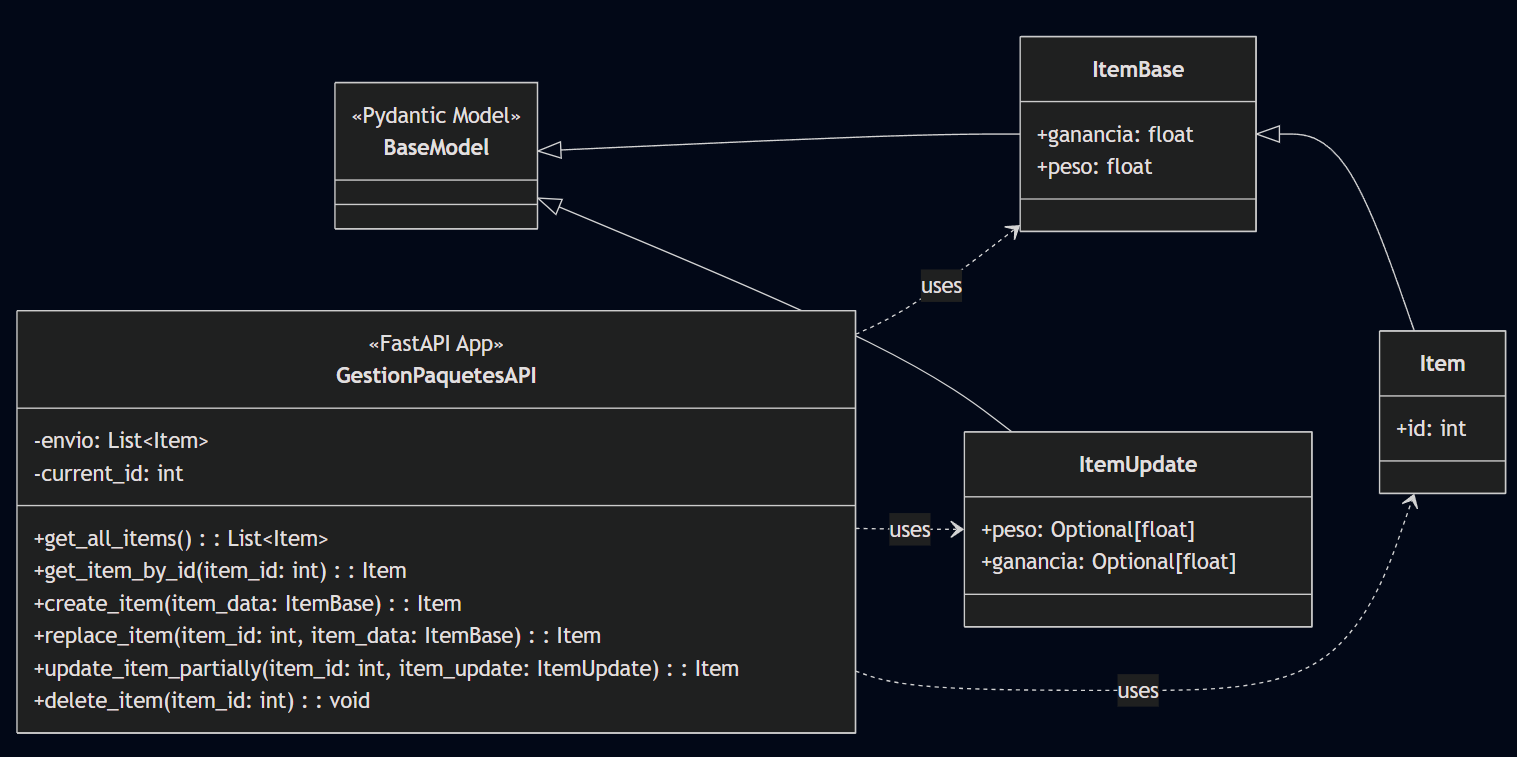
\includegraphics[width=1\textwidth]{Imagenes/Diagrama UML.png}
\end{figure}
\section{Implementación}
\begin{figure}[h!]
    \centering
    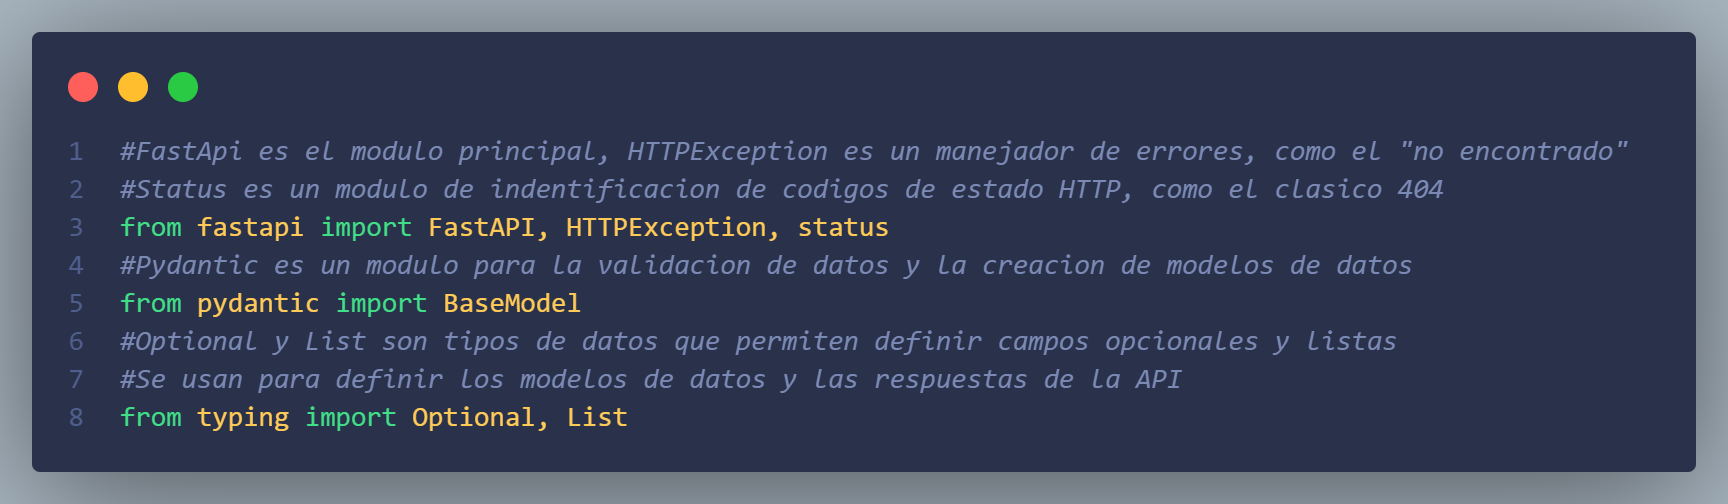
\includegraphics[width=1\textwidth]{Imagenes/Captura1_librerias.png}
\end{figure}

En este apartado se tienen los modulos a utilziar para el funcionamiento de la practica.\\
FastApi nos permite contruir APIS de manera rapida y sencilla, permitiendo definir rutas y manejar solicitudes HTTP de manera eficiente.\\
Las rutas que utilizaremos en esta practica son: GET, POST, PUT y DELETE.\\
Utilizamos Pydantic para validad entradas y para la creacion de un modelo de datos, que en es este caso sera para tener la id de un objeto, y su respectivo contenido.\\
Optional y list son tipos de datos que nos permiten definir atributos que pueden ser opcionales y listas respectivamente.\\


\begin{figure}[h!]
    \centering
    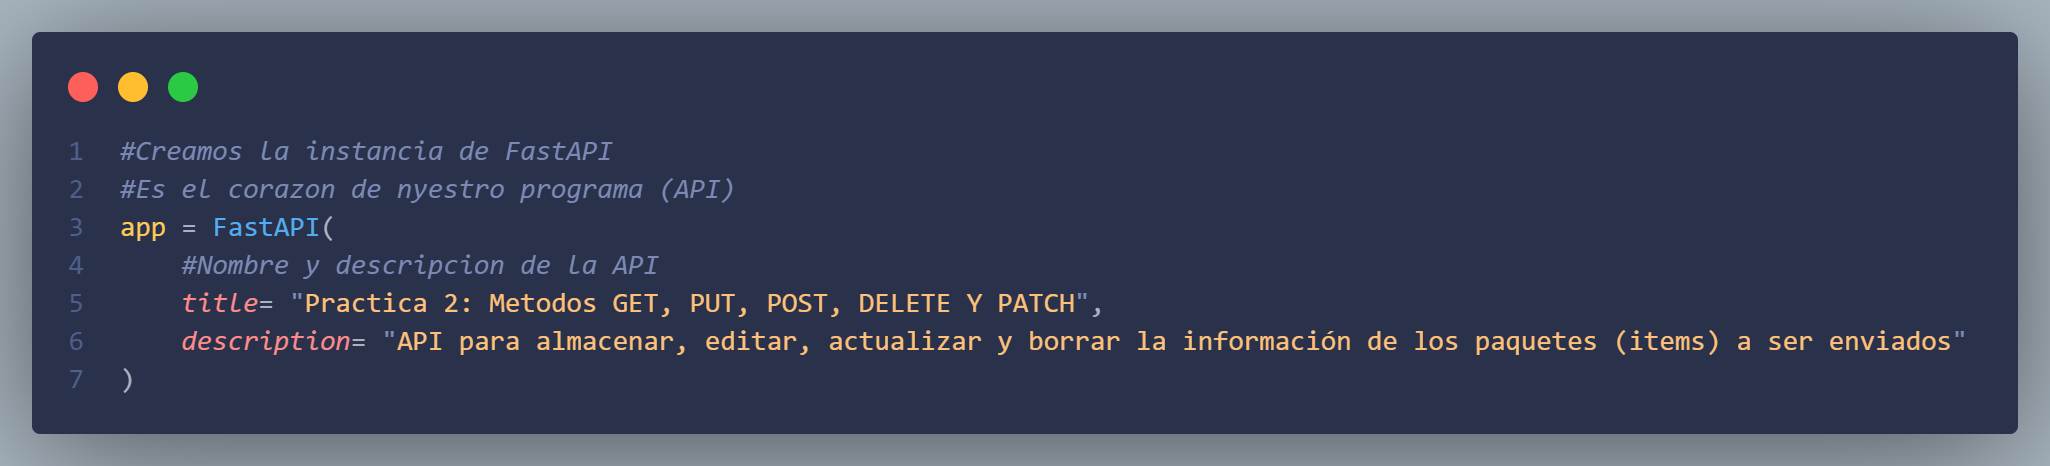
\includegraphics[width=1\textwidth]{Imagenes/Captura2_corazon del programa.png}
\end{figure}

Iniciamos con el corazon de nuestro programa, que es la instancia de FastAPI, en donde definimos el nombre y la descripcion de la API.\\

\begin{figure}[H]
    \centering
    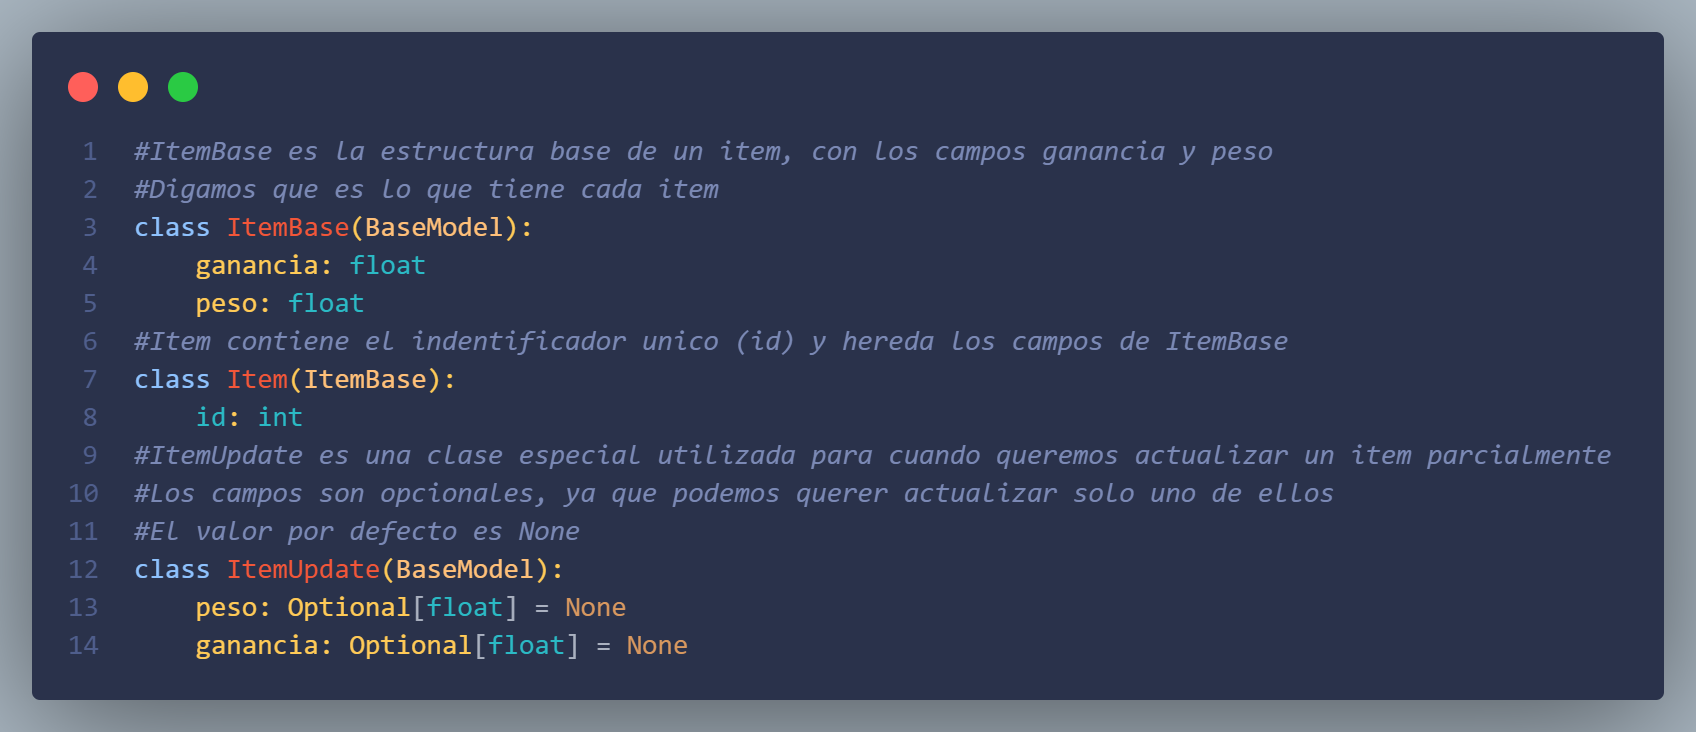
\includegraphics[width=1\textwidth]{Imagenes/Captura3_esctructuradatos.png}
\end{figure}

Gracias a Pydantic, podemos crear una estructura de datos para nuestros objetos a utilizar.
Se tiene un id de tipo entero, este servira para identificar cada objeto.
Cda objeto tiene un contenido de datos, en este caso cuenta con ganancia y perso, ambos de tipo flotante.
Además se tiene una estrcutura para actualizar los datos parcialmente, los campos son opcionales, esto es debido a que no es obligatorio actualizar ambos.

\begin{figure}[H]
    \centering
    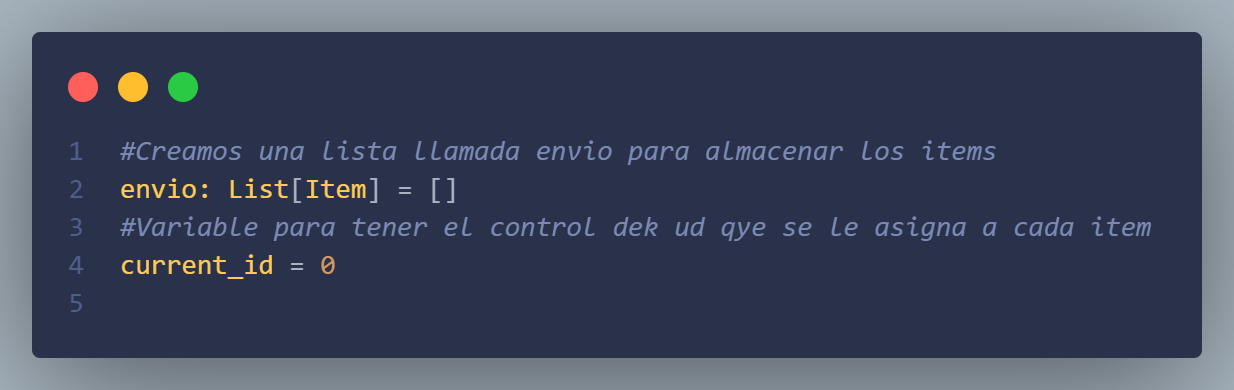
\includegraphics[width=1\textwidth]{Imagenes/Captura4_variablesGlobales.png}
\end{figure}

Utilizamos variables globales para almacenar los objetos y llevar un control del id.
El id se inicializa en 0, y se incrementa cada vez que se crea un nuevo objeto.
Los objetos se almacenan en una lista, que inicialmente esta vacia.\\

Para poder iniciar nuestra API, se debe utilizar un comando en la terminal: python -m uvicorn Codigo.Practica2:app --reload.
Existen diferentes maneras de iniciar la API, pero esta es la que se utilizo en este caso.
Una cosa interesante es que debemos especificar en el comando que trabajaremos con python, ya que sin el detecta como desconocido a uvicorn.
\begin{figure}[H]
    \centering
    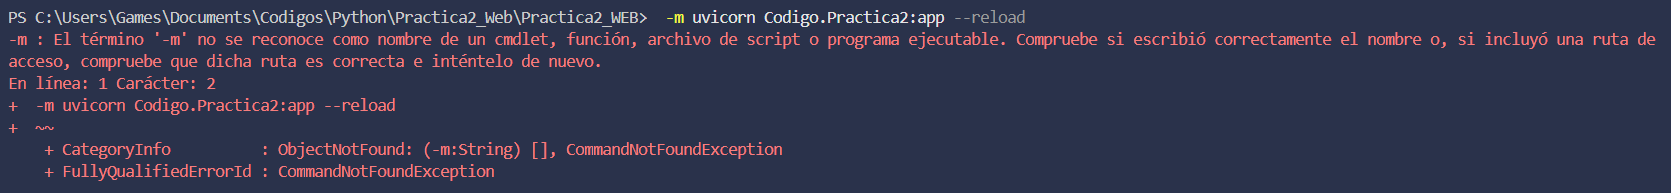
\includegraphics[width=1\textwidth]{Imagenes/Captura_consola2.png}
    \caption{Error si no se especifica que se trabajara con python}
\end{figure}

\begin{figure}[H]
    \centering
    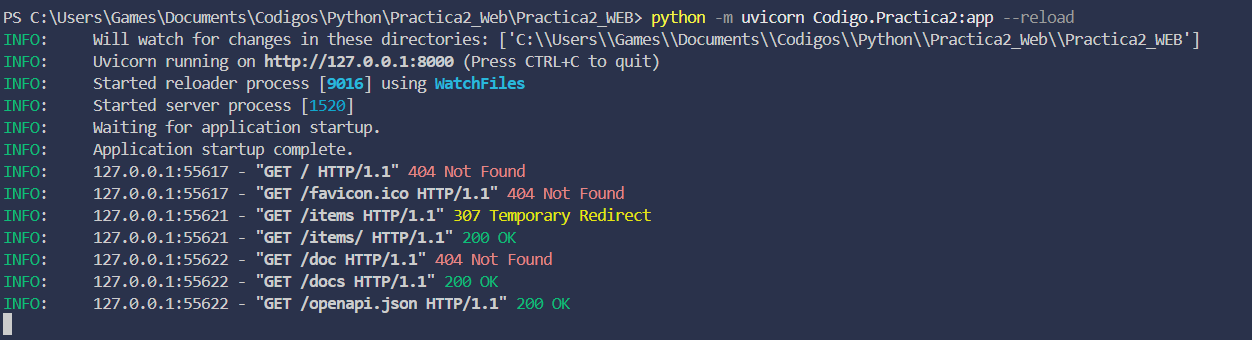
\includegraphics[width=1\textwidth]{Imagenes/Captura_consola1.png}
    \caption{Resultado correcto al iniciar la API}
\end{figure}
Cuando se inicia la api, en la consola podemos visualizar la direccion en la que se esta ejecutando, en este caso es de manera local, por lo cual se ustiliza: \url{http://127.0.0.1:8000}
Además podemos ver las peticiones que se le realizan a la pagina y si hubo un error o se realizo correctamente.

\begin{thebibliography}{99}

\bibitem{ref1} M\'etodos de petici\'on HTTP. (s/f). \textit{MDN Web Docs}. Recuperado el 23 de septiembre de 2025, de \url{https://developer.mozilla.org/es/docs/Web/HTTP/Reference/Methods}

\bibitem{ref2} Ram\'irez Monta\~no, S. (s.f.). ``Historia, dise\~no y futuro de FastAPI''. \textit{FastAPI}. Recuperado el 23 de septiembre de 2025, de \url{https://fastapi.tiangolo.com/es/history-design-future/}

\bibitem{ref3} Wikipedia. (2025, julio 11). ``FastAPI''. \textit{Wikipedia, la enciclopedia libre}. Recuperado el 23 de septiembre de 2025, de \url{https://es.wikipedia.org/wiki/FastAPI}

\bibitem{ref4} Lubanovic, B. (2019). \textit{Introducing Python: Modern Computing in Simple Packages} (2\textsuperscript{a} ed.). O'Reilly Media. ISBN: 9781492051367

\bibitem{ref5} Linode Guides \& Tutorials. (2021, agosto 6). ``Document a FastAPI App with OpenAPI''. \textit{Linode}. Recuperado el 23 de septiembre de 2025, de \url{https://www.linode.com/docs/guides/document-a-fastapi-app-with-openapi/}

\end{thebibliography}
\end{document}